\documentclass[letterpaper,ugly,10pt]{ion-gps}

  \usepackage{alltt}
  \usepackage{subfigure}
  \usepackage{graphicx}
  \usepackage{listings}

  \usepackage{amsmath}     % cases environment
  \usepackage{indentfirst} % indent all first paragraphs
  \usepackage{times}

%%%%%%%%%%%%%%%%%%%%%%%%%%%%%Commands to support toolkit apps table%%%%%%%%%%%%%%%%%%%%%%%%%%%%%%%%%%
  \usepackage{multirow}
  \usepackage{rotating}
  \usepackage{colortbl}
  \usepackage{xcolor}

  \newcommand{\sideco}{gray}
  \newcommand{\sideso}{1.0}
  \newcommand{\sidect}{gray}
  \newcommand{\sidest}{1.0}
  \newcommand{\sidewidth}{0.15in}
  \newcommand{\entco}{gray}
  \newcommand{\entso}{1.00}
  \newcommand{\entct}{gray}
  \newcommand{\entst}{0.95}
  \newcommand{\twidth}{1.0in}
  \newcommand{\dwidth}{2.3in}
  \newcommand{\ewidth}{2.3in}

   \newcommand{\appdesce}[3] {\cellcolor[\sideco]{\sideso} & \cellcolor[\entct]{\entst} \multirow{1}{\twidth}{\footnotesize{#1}} & \cellcolor[\entct]{\entst} \multirow{1}{\dwidth}{\footnotesize{#2}} & \cellcolor[\entct]{\entst} \multirow{1}{\ewidth}{\ttfamily{\footnotesize{#3}}}}

   \newcommand{\appdesco}[3]{\cellcolor[\sideco]{\sideso} & \cellcolor[\entco]{\entso} \multirow{1}{\twidth}{\footnotesize{#1}} & \cellcolor[\entco]{\entso} \multirow{1}{\dwidth}{\footnotesize{#2}} & \cellcolor[\entco]{\entso} \multirow{1}{\ewidth}{\ttfamily{\footnotesize{#3}}}}
%%%%%%%%%%%%%%%%%%%%%%%%%%%%%%%%%%%End commands to support apps table%%%%%%%%%%%%%%%%%%%%%%%%%%%%%%%%%
  \newcommand{\bkup}{-2}
  \newcommand{\execsize}{\scriptsize}
  \newcommand{\sidesize}{\small}

  \newcommand{\gpstkapp}[1]{\textit{\mbox{#1}}}
  \newcommand{\gpstkdir}[1]{\texttt{\mbox{#1}}}
  \newcommand{\gpstkcommand}[1]{\texttt{\mbox{#1}}}
  \newcommand{\gpstkclass}[1]{\texttt{\mbox{#1}}}
  \newcommand{\rinexobservable}[1]{\texttt{#1}}

%  \usepackage{newcent}
%%%%%%%%%%%%%%%%%%%%%%%%%%%%%%%%%%%%%%%%%%%%%%%%%%%%%%%%%%%%%%%%%%%%%%%%%%%%%%%
% Title
%%%%%%%%%%%%%%%%%%%%%%%%%%%%%%%%%%%%%%%%%%%%%%%%%%%%%%%%%%%%%%%%%%%%%%%%%%%%%%%

\title{\huge\bf The GPSTk: New Features, Applications, and Changes }

\author{ R. Benjamin Harris, Tracie Conn, Thomas Gaussiran, 
Chris Kieschnick, Jon Little, Richard Mach, \\
David Munton, Brent Renfro, Scot Nelsen, Brian Tolman, Jonathan Vorce \\
       \it{Applied Research Laboratories, The University of Texas at Austin} \\
	\\
	Dagoberto Salazar \\
	\it{Grupo de Astronomia y Geomatica, Universitat Polit\`{e}cnica de Catalunya} }

\date{}

% This becomes footer if defined
%\conference{}
\conference{\emph{First presented at ION GNSS 2007, Sept. 25 to 28, 2007, Fort Worth, Texas}}

%%%%%%%%%%%%%%%%%%%%%%%%%%%%%%%%%%%%%%%%%%%%%%%%%%%%%%%%%%%%%%%%%%%%%%%%%%%%%%%
% Defines
%%%%%%%%%%%%%%%%%%%%%%%%%%%%%%%%%%%%%%%%%%%%%%%%%%%%%%%%%%%%%%%%%%%%%%%%%%%%%%%

\newcommand{\br}{\mbox{\boldmath $r$}}
\newcommand{\bv}{\mbox{\boldmath $v$}}
\newcommand{\be}{\mbox{\boldmath $e$}}
\newcommand{\bzero}{\mbox{\boldmath $0$}}
\newcommand{\bomega}{\mbox{\boldmath $\omega$}}
\newcommand{\bK}{\mbox{\boldmath $K$}}
\newcommand{\bx}{\mbox{\boldmath $x$}}
\newcommand{\ba}{\mbox{\boldmath $a$}}
\newcommand{\bI}{\mbox{\boldmath $I$}}
\newcommand{\bPhi}{\mbox{\boldmath $\Phi$}}
\newcommand{\bH}{\mbox{\boldmath $H$}}
\newcommand{\bR}{\mbox{\boldmath $R$}}
\newcommand{\bQ}{\mbox{\boldmath $Q$}}
\newcommand{\bP}{\mbox{\boldmath $P$}}

\definecolor{console}{rgb}{0.90,0.90,0.90}
\lstset{basicstyle=\ttfamily, backgroundcolor=\color{console}}

%%%%%%%%%%%%%%%%%%%%%%%%%%%%%%%%%%%%%%%%%%%%%%%%%%%%%%%%%%%%%%%%%%%%%%%%%%%%%%%
% Body
%%%%%%%%%%%%%%%%%%%%%%%%%%%%%%%%%%%%%%%%%%%%%%%%%%%%%%%%%%%%%%%%%%%%%%%%%%%%%%%

\begin{document}

\def\figurename{Fig.}
\def\tablename{Table}

\pagestyle{plain} % Page number on back of paper with hand written in pencil
%\pagestyle{fancy}

\maketitle

%\thispagestyle{empty} % empty pagestyle for the title page

% This turns off all page numbers -- required for version turned into the ION
%\pagestyle{empty}

\section*{Biography}

R. Benjamin Harris is an Engineering Scientist at \mbox{Applied Research
Laboratories}, The University of Texas at Austin (ARL:UT). He received a B.S. in Aerospace Engineering from the University of Texas at Austin (UT Austin) (1994), and is a Ph.D. candidate in the same department. He received an M.S. in Aeronautics and Astronautics from \mbox{Stanford (2000)}.

Tracie Conn is an Engineering Scientist Associate at ARL:UT. She
graduated with a B.S. in Aerospace Engineering from UT Austin (2006).

Thomas Gaussiran is the director of the Space and Geophysics Laboratory
(SGL) at ARL:UT. He received his B.S. in Physics from UT Austin (1988)
and M.S. (1991) and PhD. (1994) from Rice University.

Chris Kieschnick is an undergraduate majoring in Computer Science at UT Austin.

Jon Little is a Senior Engineering Scientist at ARL:UT. He obtained a
B.S. (1988) and a M.S. (1990) from Auburn.

Richard Mach is a project lead at ARL:UT.  He has been involved with
GPS applications since 1990.  He holds a B.S. (1990) and M.S. (1992) in Aerospace
Engineering from UT Austin.

David Munton is a Research Associate at ARL:UT. He earned a B.S. in Physics from Sonoma State University (1982), and a Ph.D. in Physics from UT Austin (1992). 

Scot Nelsen is an Engineering Scientist at ARL:UT. He earned a B.S. in
Electrical Engineering at UT Austin (1998).

Brent Renfro is a program manager at ARL:UT.  He has a B.A. in Physics from Wabash College (1979) and a M.A. in Computer Science from UT Austin (1983).

Brian Tolman is a Research Scientist at ARL:UT. He holds a
Ph.D. in theoretical physics from UT Austin (1982).

Jonathan Vorce is an undergraduate majoring in Aerospace Engineering at UT Austin.

Dagoberto Salazar is an Aeronautical Engineer (IUPFAN, Venezuela, 1992). After working several years both for government and private industry, he pursued postgraduate studies in Instrumentation and Control (UCV). He is currently a Ph.D. candidate in Aerospace Science and Technology at the Universitat Polit\`{e}cnica de Catalunya (UPC, Spain).

\section*{Abstract}
The GPS Toolkit, or GPSTk, is an open source project that provides a
software suite to the GNSS community. The goal of the project is to
free researchers to focus on research, not lower-level
coding. The suite is composed of a library and a suite of
applications built on the library.

Since the GPSTk was last presented at the ION GNSS 2006, the project has grown in scope and user base. Metrics provided by service providers SourceForge and Google quantify that growth. To accommodate the increase in demand and code complexity, the documentation system has been replaced with a community-managed website or wiki. The project has customized the wiki to support documentation commonly associated with GNSS software development.

Because the project is open source, new contributions are key to its success. The library has been reorganized to preserve contributions that are experimental or application specific. The new organization preserves usability and stability of the library's core functionality. The core library has been modified as well. Data structure and almanac processing classes have been added. New applications have also been contributed. This includes two suites of applications, one that simulates tracking the GPS signal and another that analyzes range residuals.


\section*{Introduction}

The goal of this paper is to familiarize the reader with the purpose, status, and future direction of the GPSTk project. The overall capabilities of the applications and library are briefly restated. New capabilities are discussed in detail. Examples of projects based on the GPSTk are described. 

\section*{Project Summary}

The goal of the GPSTk project is to provide a open source library and suite of applications to the satellite navigation community to free researchers to focus on research and not lower level coding.

GPS users employ practically every computational architecture and operating system. Therefore, the design of the GPSTk suite is as platform-independent as possible. Platform independence is achieved through use of the ISO-standard C++ programming language~ \cite{iso-14882-2003}. The principles of object-oriented programming are used throughout the GPSTk code base in order to ensure that the code is modular, extensible, and maintainable.

The GPSTk suite is composed of a library and a set of
applications built on the library. The library provides a wide array of functions that solve processing problems associated with GPS such as the navigation solutions or reading standard formats such as RINEX. The applications support a greater depth of functionality. Each application implements a specific GNSS processing task.

\subsection*{Getting the GPSTk}

The GPSTk can be downloaded over the web via links provided on the project
website, http://www.gpstk.org/ . Precompiled binaries are available for many platforms. 
Access to the latest code base is provided through a
publicly accessible repository hosted by SourceForge.  The repository is 
accessed using the \gpstkapp{Subversion} utility.  \gpstkapp{Subversion} is a
open source version control system that coordinates development among
users over the Internet \cite{subversion, subversionbook}.

\gpstkapp{Subversion} is a console application that operates identically on a number
of operating systems.  The following command can be used to retrieve the
latest GPSTk source from SourceForge and write it into a directory structure on
the user machine in the current working directory:

\begin{scriptsize}
\begin{lstlisting}
svn co https://gpstk.svn.sourceforge.net/svnroot/gpstk
\end{lstlisting}
\end{scriptsize}

Note that it is not necessary to provide any user information or password to retrieve the code.
This form of access is referred to as anonymous in the \gpstkapp{Subversion} documentation.
Any directory in this structure can be updated to the latest code by first making it the 
current working directory then executing the following command:

\begin{scriptsize}
\begin{lstlisting}
svn update
\end{lstlisting}
\end{scriptsize}


\subsection*{Project Documentation} 

The GPSTk project's web site was initially hosted by SourceForge. It contained static content which was difficult to update. To facilitate true cross organizational development and user interaction, ARL:UT established a dynamic website, also known as a wiki.

The wiki site utilizes an open source product called \mbox{TWiki \cite{twiki}} that is not only a wiki but a full featured and easily extensible development platform. The project has customized the base TWiki installation to add two capabilites. One capability allows for users to submit questions or answers about the project. Another provides a framework for capturing development documentation, such as brainstorming or designs. The site also supports the \LaTeX \vspace{1mm} format allowing for expressive content such as equations. Finally, users can choose to be notified when topics are changed via email or web feed.

The website hosts a copy of the Doxygen documentation.  This documentation  is updated from the code repository on a daily basis to ensure easy access to the latest documentation changes.  Additionally, an IRC channel was established to create a real-time avenue of developer communication.  Finally, the new website contains new documentation that describe the GPSTk development process, the release process, how to get started with the GPSTk, and more.  The goal of this added information was to help new developers become familiar with the project operation so they can become effective contributors.

Currently, the website hosts a PDF version of the GPSTk users manual.  For the next revision of the manual, ARL:UT plans to convert it to a set of wiki pages. Then users will not only be able to update the manual, but also generate an offline copy of it using TWiki's PDF generation capability.

\subsection*{Project Activity Metrics}

To give a brief insight into the number and diversity of visitors to the new wiki site, the following information was extracted from Google Analytics by looking at the traffic over the past 7 months.  The website has seen on average over 1500 visits per month with over 1000 unique visitors per month. Visitors locate the website directly (about 30\% of the time), by following a link from an other site (about 42\% of the time), and by search engines (about 28\% of the time).  The website has seen visitors from 124 countries or territories with the top 10 countries of visitors being the United States, Germany, China, United Kingdom, Taiwan, Italy, Canada, Australia, Spain, and France. Approximately 30\% of all vistors return to the website after the first visit.  Figure~\ref{fig:googleanalytics} shows the distribution of visit worldwide.
%
\begin{figure*}
	\centering
	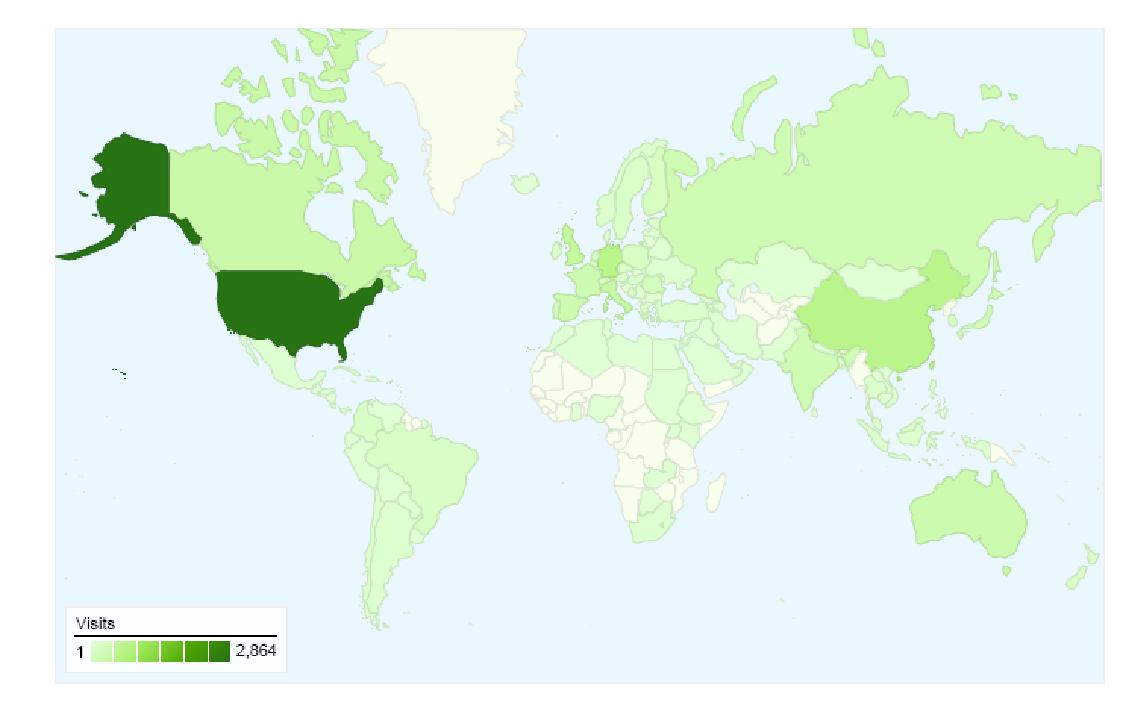
\includegraphics[width=6in,bb=0 0 535 329]{gpstk-google-analytics.eps}
% gpstk-google-analytics.eps: 300dpi, width=4.53cm, height=2.79cm, bb=0 0 535 329
	\caption{Website visitor distribution, March to September 2007, courtesy Google Analytics}
	\label{fig:googleanalytics}
\end{figure*}

The activity of the project is measured by SourceForge as well. SourceForge tracks project activity for each service it provides: web traffic, Subversion transactions, file downloads, bug entries, and more. This facility reports that the GPSTk binary packages have been downloaded more than 10,000 times from September, 2006, to the time of this writing, September 2007. The activity metrics can also be investigated over time. Two metrics are displayed in Figure~\ref{fig:sfactivity}. The number of packages downloaded per month rate has remained fairly constant while the amount of SourceForge traffic for the project has declined. It can be inferred that the project TWiki has offloaded traffic from the SourceForge site. The spike in February, 2007, has yet to be explained.

%
\begin{figure}
	\centering
	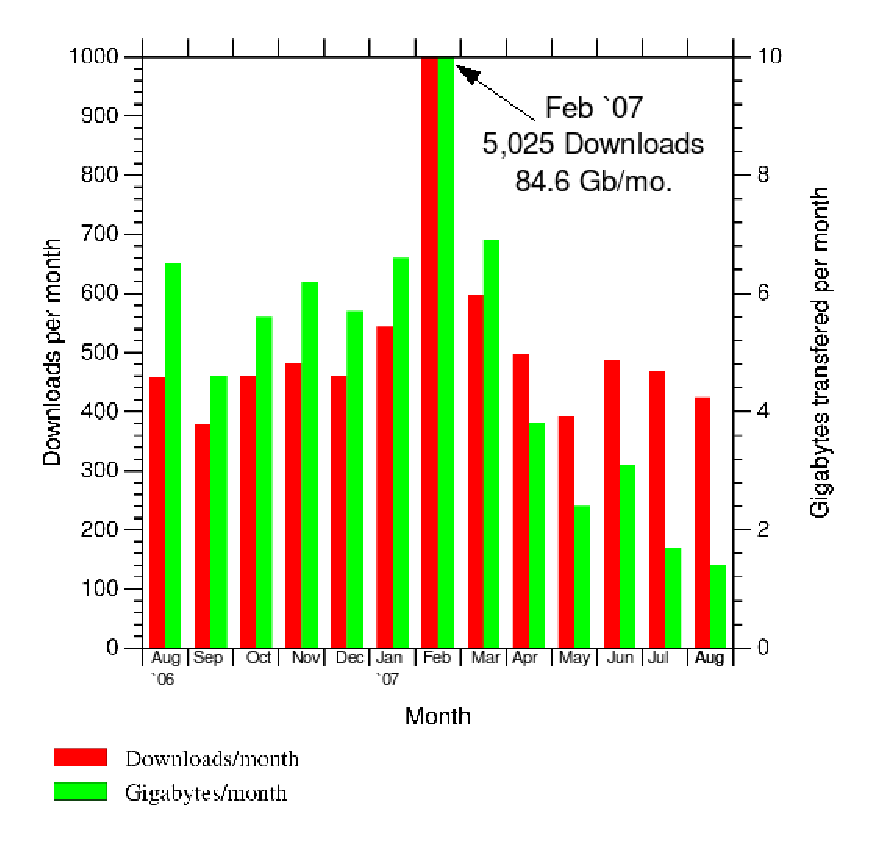
\includegraphics[bb=0 0 402 389,width=3.3in]{sfdownloadstouched.eps}
% sfdownloadstouched.eps: 300dpi, width=3.40cm, height=3.29cm, bb=0 0 402 389
	\caption{Project activity through SourceForge site}
	\label{fig:sfactivity}
\end{figure}

Two final metrics of project activity relate to the size and value of the code base. Version 1.3 of the GPSTk contains approximately 200,000 source lines of code. In comparison, version 1.2 contained 150,000 source lines of code. Version 1.1 contained 70,000. The value of the code base can also be estimated using the COCOMO model, which was first developed to manage aerospace software developments \cite{cocomomodel}. According to the COCOMO model, the estimated value of version 1.3 of the GPSTk source code is \$7 million. These size and value metrics were generated using David A. Wheeler's SLOCCount utility \cite{sloccount}.

\subsection*{Testing and the Release Process}

As discussed in prior ION papers \cite{ion:gnss06}, testing of the \mbox{GPSTk library} is designed with three distinct goals in mind: testing is repeatable with a low amount of effort, testing is distributed along with the library to support both internal regression testing and to assure outside users and contributors of the quality of the library, and testing is designed to accommodate easy additions to the existing test suite.  These goals have been retained, though the amount of the library that is covered by the test suite is expanding rather more slowly than anticipated. 

Part of the reason for that slow expansion is the realization that testing is only one part of an overall release process.  Following the move to on-line source management in July 2006 \cite{ion:gnss06}, the project has invested effort in defining and automating the release process. The release process is the process by which a stable and reviewed version of the code is first extracted from the Subversion repository, then tested for quality. The ability to conduct the release process smoothly is critical to user support.

\section*{Functional Summary}

\subsection*{Library Functionality}

The GPSTk library provides the base functionality for the GPSTk applications and for a number of other independent projects. There are several categories of functions:

\begin{itemize}
\item RINEX manipulation
\item Time conversion, manipulation and storage
\item Matrix computation
\item Basic transforms of time and location
\item Precise ephemeris processing
\item Range prediction and error modeling
\item Reference frame computations
\item Statistics
\item Troposphere delay models
\item Earth orientation transforms
\item FIC processing
\item Almanac processing
\item Low level BINEX input and output
\item Broadcast ephemeris processing
\item Clock models
\item Code generation
\item Cycle slip and discontinuity correction
\item Expression evaluation
\item Numerical integration
\item Combinations and difference computations
\item Data structures
\item Navigation solution
\end{itemize}

A more detailed description of the functionality provided by the GPSTk library is generated from the code using the Doxygen utility \cite{doxygen}. An updated image of that documentation is kept on the GPSTk website \cite{gpstkwebsite}. A number of prior presentations, articles and papers discuss the capabilities of the library in more detail \cite{lj04,ion:gnss04,ion:gnss05,ion:gnss06,gpssolutions2007}.

\subsection*{Application Functionality}

A number of GPSTk applications are cross-platform. These applications are used to form the precompiled binary releases. The version 1.3 cross-platform applications are listed in Table~\ref{apptbl}. They are sorted into groups by their general 
purpose. Each row describes one GPSTk application or toolchain. A more detailed description of the applications can be found in References \cite{ion:gnss06} and \cite{gpssolutions2007}.

\begin{table*}
	\centering
	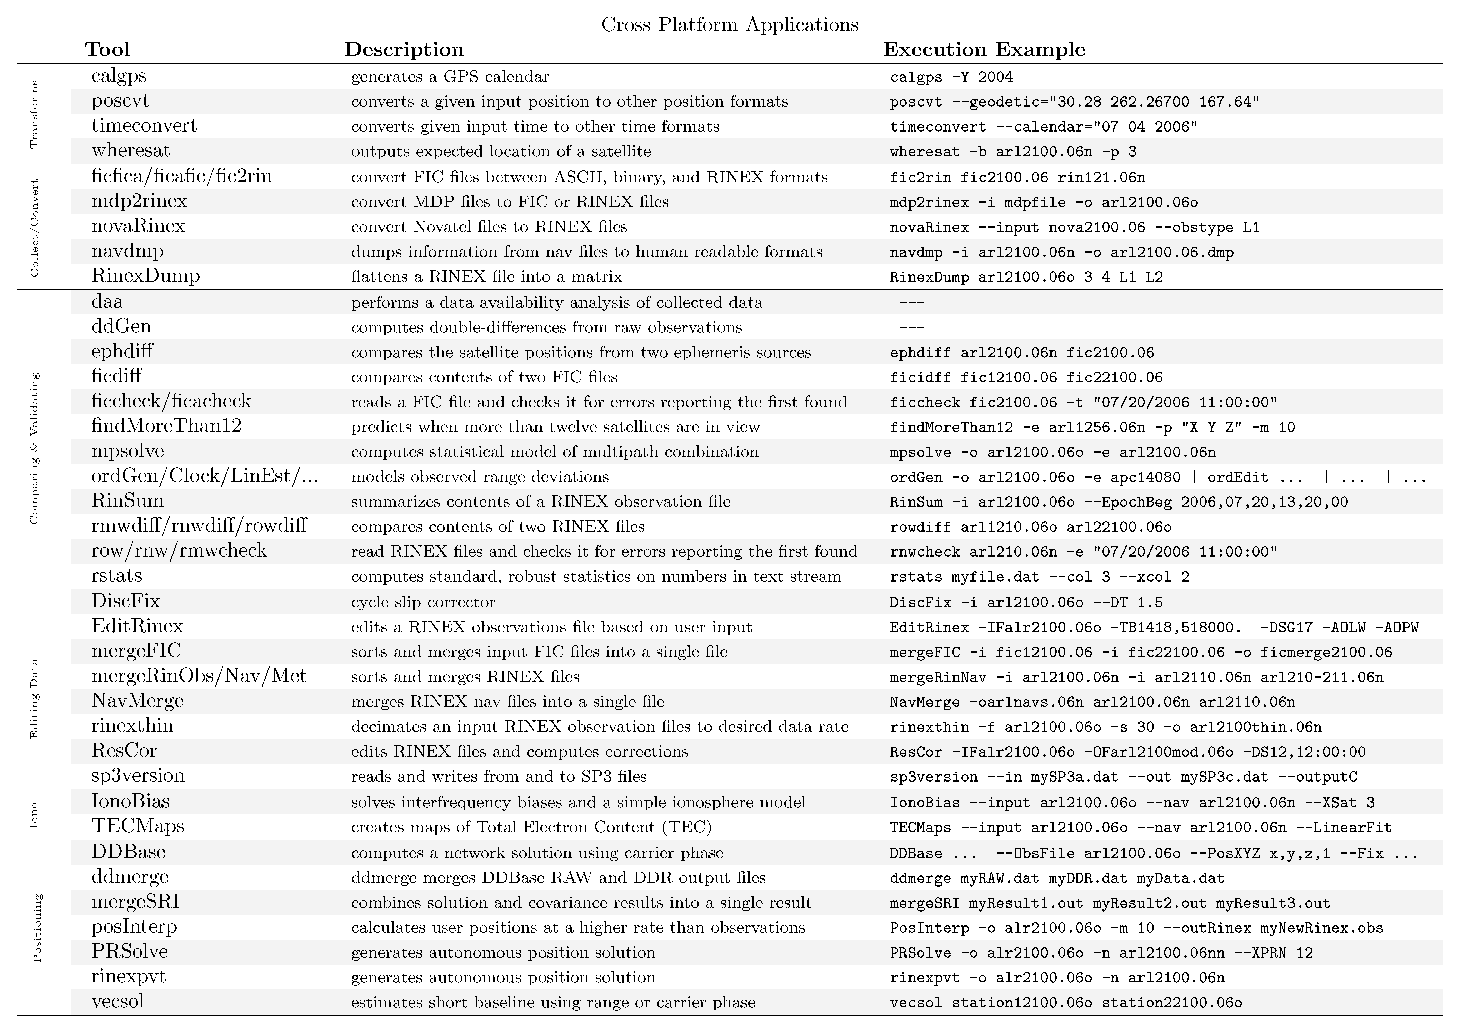
\includegraphics[width=9in,angle=90,bb=57 73 742 554]{crossplatformapps.eps}
% toolkitapps.eps: 300dpi, width=5.71cm, height=4.38cm, bb=57 52 731 569
	\caption{Cross platform applications.}
	\label{apptbl}
\end{table*}

\begin{table*}
\centering
\begin{tabular}{ll} \hline \hline
Source Location &  Function \\ \hline
\gpstkdir{dev/apps/bindings} & Interfaces to Perl, Java, and other languages. \\
\gpstkdir{dev/apps/swrx} & Simulation of the GPS signal and receiver tracking. \\
\gpstkdir{dev/apps/RinexPlot} & Plotting observation combinations. Written in perl-Tk. \\
\gpstkdir{dev/apps/MDPtools} & Processing TCP/IP or file-based observations in the MDP format.\\
\gpstkdir{dev/apps/receiver} & Capture of data from an Ashtech receiver. \\ \hline \hline 
\end{tabular}
\caption{Applications with dependencies outside standard C++}
\label{apptbl2}
\end{table*}

In contrast, other GPSTk applications are broadly useful but require more than the standard C++ environment to compile. These applications are summarized in Table~\ref{apptbl2}.


\section*{Recent Enhancements}

\subsection*{Yuma and SEM Almanac Processing}

When performing GPS mission analysis or processing observations that span multiple months, an application may need to model the state of the constellation. Two publicly available formats provide this information, Yuma \mbox{ \cite{yumaformat}} and \mbox{SEM \cite{semformat}}. Classes have been added to the core library of the GPSTk to process almanacs in these formats.

\subsection*{Library Restructuring}

The core of the GPSTk is the library, and its source is located in the \gpstkdir{dev/src} directory. This directory contains classes, algorithms, and data that are fundamental to GNSS processing and should compile on any system with a compiler that conforms with the international standard for C++ \cite{iso-14882-2003}. Often, however, the GPSTk contains code that could be useful in GNSS processing but do not fit this description. A number of such cases are present throughout the code base. The code could contain highly specialized algorithms, or be related to the message format of a specific receiver. The code could require libraries or system functions that are broadly available but not part of the C++ standard. To preserve code of this nature, the GPSTk project has introduced a new directory structure. This new code base is located in the \gpstkdir{dev/lib} directory. The GPSTk source directory structure is illustrated in Figure \ref{fig:gpstkdevstructure}.
\begin{figure}
	\centering
	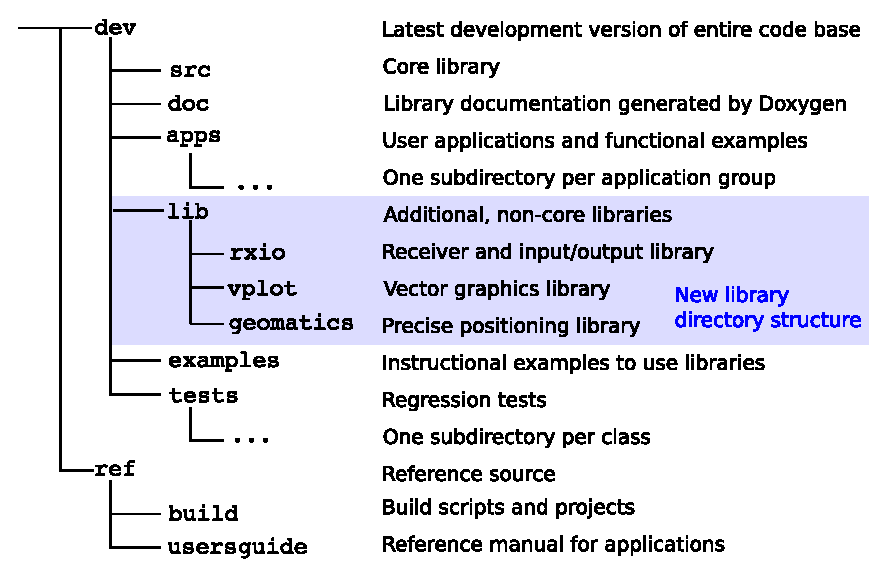
\includegraphics[width=3.2in,bb=91 373 500 634]{gpstk-directory-structures.eps}
% gpstk-directory-structures.eps: 300dpi, width=3.35cm, height=2.21cm, bb=91 373 487 634
	\caption{Directory structure for GPSTk source}
	\label{fig:gpstkdevstructure}
\end{figure}

The guidelines for adding to the \gpstkdir{dev/lib} directory are similar to the rules for the \gpstkdir{dev/apps} directory. Anything that is related to GNSS is acceptable. The intent is to encourage experimentation and development of new ideas. No files are directly placed in \gpstkdir{dev/lib} and subdirectories are created to group related items. Subdirectories can have dependencies upon third party libraries and platform specific extensions. These subdirectories may depend upon the core GPSTk library (in \gpstkdir{dev/src}) but they may not depend upon anything in \gpstkdir{dev/apps}. More importantly, nothing in the core GPSTk library may depend upon items in \gpstkdir{dev/lib}. This last point is imperative to maintain the portability and broad support of the GPSTk core library.

While anything GNSS related can be added under the \gpstkdir{dev/lib} directory, the same is not true of the build process. It should only include items that will generally compile. To facilitate compiling the items in the new directory, the build will recurse into \gpstkdir{dev/lib} by default. Just like in \gpstkdir{dev/apps}, subdirectories that are listed in \gpstkdir{dev/lib Jamfile/Makefile} will be built when the build is invoked from the \gpstkdir{dev} directory. This also allows applications to be built and linked against the items under the \gpstkdir{dev/lib} directory.  While this guidance is somewhat vague, it does imply that the author is intending to keep the build from breaking under the common platforms that the GPSTk is used under (Linux/gcc and Windows/Visual C++). While the default build process will not recurse into every directory in \gpstkdir{dev/lib} and \gpstkdir{dev/apps}, individual directories may be built and installed manually. This is how libraries and applications that are platform specific are built and installed.

There are three subdirectories within \gpstkdir{dev/lib}: \gpstkdir{rxio}, \gpstkdir{geomatics}, and \gpstkdir{vplot}. The directory \gpstkdir{rxio} contains \gpstkclass{FFStream} definitions for the MDP receiver data type. The directory \gpstkdir{vplot} contains a set of plotting routines. The \gpstkdir{geomatics} directory contains precise positioning algorithms. Currently, there are several items that are in \gpstkdir{dev/src} that are candidates to be moved to the \gpstkdir{dev/lib} directory structure. Examples are the FIC and SMODF parsing routines as these formats are only used by a very small community.

\subsection*{Observed Range Deviation Toolchain}
An Observed Range Deviation (ORD) is defined as the difference between an observed pseudorange and its predicted value \cite[p.465]{ps:gta}. A number of algorithms and terms are required to compute both the observed and predicted pseudoranges. Both can be corrected for known effects such as relativity, earth rotation and atmospheric delay. When all of these effects are accounted for, ORDs can be in the 10-30 cm range for a dual-frequency, geodetic quality receiver.

Prior to version 1.3 of the GPSTk, the \gpstkapp{reszilla} application provided the capability to compute ORDs from GPS pseudorange, carrier phase, and Doppler data. However, as of fall 2006, \gpstkapp{reszilla} had become quite complex and difficult to maintain. The program has since been redesigned into a suite of smaller applications that can be used in conjunction. Such a set of applications is often referred to as a \emph{toolchain}.

The new applications are designed to be modular so that the output of one program can be used as the input to the others. The input and output can be captured to file, or streamed between applications in real time. In all of the platforms supported by the GPSTk, these two modes of are supported by redirection and piping. In UNIX and Windows command line environments, the redirect operator \gpstkcommand{>} captures standard output to a file. For example, 
\gpstkcommand{calgps > calendar.txt} writes a simple text based GPS calendar for the current month to a file \gpstkdir{calendar.txt}. Piping is supported by the pipe operator \gpstkcommand{|}. An example of piping in the Windows command line environment is the command \gpstkcommand{calgps -Y 2004 | more }. By allowing the user to choose how to connect this toolchain, the new design allows for greater flexibility and ease of use. There are currently six tools that both replace and enhance the ORD computation capability of \gpstkapp{reszilla}: \gpstkapp{ordGen}, \gpstkapp{ordEdit}, \gpstkapp{ordClock}, \gpstkapp{ordLinEst}, \gpstkapp{ordStats}, and \gpstkapp{ordPlot}.

The tool that must be run first in the chain is \gpstkapp{ordGen}. Via command line options and data in a variety of file formats, the program accepts an antenna position, observation data, ephemeris information and weather data. The position is assumed to be a very accurate, surveyed location. The user may also specify which combination of observations are to be used, such as C/A-Code only or P/Y-Code on L1 and L2. ORD's will be flagged if the data seems erroneous based on several criteria: low signal strength, extremely large pseudorange, large tropospheric correction, SV elevation below the horizon, or indication of bad SV health in subframe 1 of a valid 6-bit SV health bitfield. The ORD solutions for each SV are output in a format readable by the other ORD tools; it is called the ORD file.

The next tool that may be used is \gpstkapp{ordEdit}. This program removes lines from the ORD file based on various criteria. Data may be filtered based on time, SV elevation, SV heath, or PRN number. 

For many GPS receivers, the most significant effect to account for when correcting the observed range is the receiver clock offset, or the difference between a receiver's internal time and true GPS time.  \gpstkapp{ordClock} makes an estimate of the receiver clock offset by averaging the ORDs of all SVs for each epoch. The bias can be optionally removed from the ORDs for each epoch. These clock parameters may then be processed by \gpstkapp{ordLinEst} to compute a linear clock model estimate. A natural byproduct of forming the linear model are deviations from the model, also known as \emph{clock residuals}. Clock residuals are output by \gpstkapp{ordLinEst}.

The ORD file can be processed by \gpstkapp{ordStats} to summarize error statistics. The total number of ORDs and epochs that were flagged as erroneous are counted. For a set of user-specified elevation ranges, the standard deviation, mean and maximum values of the ORDs is listed, as well as the number of observations and the number flagged as erroneous. Looking at the results for each elevation bin is useful as ORDs tend to be much a higher when satellites are lower on the horizon.

Finally, \gpstkapp{ordPlot} is a Python \cite{python} script that uses matplotlib \cite{matplotlib} to plot ORDs, clock offsets, linear clock models and clock model residuals. Basic graph properties may be specified, and the the final image may be saved in a number of raster- and vector- based image formats. Figure~\ref{fig:ordplotoutput} is an example residual plot generated by \gpstkapp{ordPlot}.
\begin{figure*}
	\centering
	\includegraphics[bb=0 0 1200 900,width=5in]{samplePlot.eps}
% samplePlot.eps: 300dpi, width=10.16cm, height=7.62cm, bb=0 0 1200 900
	\caption{Observed range deviations computed by the ORD toolchain}
	\label{fig:ordplotoutput}
\end{figure*}

An example command line is shown below. In this example, observations are provided in the RINEX format and ephemeris information is provided as precise ephemerides. The results are edited using health information from a RINEX navigation message file and an elevation mask of ten degrees. A statistical summary is written to a text file. Finally, a PNG file is created with a plot of residuals and clock offsets. Note the use of pipes to complete the overall analysis procedure.

\begin{scriptsize}
\begin{lstlisting}
ordGen -o sample001.07obs -e apc14080 -e apc14081 
-e apc14082 | ordEdit -e sample001.07nav -m 10 | 
ordClock | ordLinEst | ordStats -o sampleStatsFile.txt |
ordPlot -s samplePlot.png
\end{lstlisting}
\end{scriptsize}


\subsection*{Toolchain to Prototype Software Receivers}

The \gpstkdir{dev/apps/swrx} directory contains classes and applications that simulate various parts of a GPS receiver. While this code has much of the functionality of a software GPS receiver, it is not intended to be a true software receiver. It is intended to be a research tool that is useful in understanding the formation of GPS signals, sampling them, tracking them, and forming observables. There are currently five separate applications in the \gpstkapp{swrx} directory: \gpstkapp{gpsSim}, \gpstkapp{codeDump}, \gpstkapp{plot}, \gpstkapp{tracker}, \gpstkapp{corltr}, and \gpstkapp{iqdump}. As with other applications in the GPSTk, the swrx applications are a command-line toolchain. The command to plot the correlation curve of the P code on PRN 1 is listed below. The resulting plot is shown in Figure~\ref{fig:swrxcorrcurve}.

\begin{scriptsize}
\begin{lstlisting}
gpsSim -q 2 -t 2e-3 -c p:1:1:50:0:p | 
corltr -q 2 -c p:1:1:0:0 | plot
\end{lstlisting}
\end{scriptsize}

\begin{figure}
	\centering
	\includegraphics[bb=120 0 1130 632,width=3.8in]{swrx-plot.eps}
% swrx-plot.eps: 300dpi, width=9.25cm, height=5.35cm, bb=0 0 1093 632
	\caption{P-Code correlation curve}
	\label{fig:swrxcorrcurve}
\end{figure}

The \gpstkapp{gpsSim} application simulates the digital output of the RF front end of a heterodyning GPS receiver. It first generates the RF signal for each code and carrier combination requested in the command line options. This RF signal can include the C/A- and/or P-Code, a 50 Hz square wave for the navigation bit transitions, a code offset, and a Doppler offset. This RF signal is then mixed with a local oscillator to form an IF and quantized to form in-phase and quadrature samples. These samples are then output as defined in the \gpstkclass{IQStream} specified.

The \gpstkapp{tracker} application implements a Costas tracking loop on an \gpstkclass{IQStream} for a single code and carrier combination. The signal to be tracked is specified on the command line and includes a time and Doppler offset. While it can acquire phase lock without exact aiding, it does not implement any explicit acquisition algorithm. This tracker aligns the integrate and dump intervals with the nav bit transitions, demodulates the navigation data, and outputs the subframes of the navigation message.

The \gpstkapp{corltr} application generates a local replica of the GPS signal and cross correlates this against the input \gpstkclass{IQStream}.

The \gpstkapp{codeDump} application simply dumps a section of the specified GPS spreading code. Its purpose is to verify code generation in the \gpstkclass{CodeGenerator} classes against the IS-GPS-200 \cite{isgps200}. This application currently only outputs C/A- or P- Code.

The \gpstkapp{plot} application is a Python script that uses matplotlib to graph the outputs of \gpstkapp{tracker}, \gpstkapp{corltr}, and \gpstkapp{codeDump}.

The \gpstkapp{iqdump} application reads in a \gpstkclass{IQStream} and dumps it as text to standard output. It also has an option to compute the percentage of time various bits are set.

Several classes form the source to the \gpstkapp{swrx} applications. The \gpstkclass{CodeGenerator} class is an abstract class that defines the interface to a pseudorandom ranging code. The intent is to make an interface that is similar to what could be easily built in hardware. The \gpstkclass{CACodeGenerator} is an implementation of the GPS C/A-Code that uses the \gpstkclass{ConstLinearRecurrentSequence} class. The \gpstkclass{PCodeGenerator} class generates the GPS P-Code. This class currently uses the P-Code generator that is in \gpstkdir{dev/src} but needs to be rewritten to use the \gpstkclass{ConstLinearRecurrentSequence} class. The \gpstkclass{ConstLinearRecurrentSequence} is a simulation of a linear feedback shift register. The \gpstkclass{SVSource} class is a simulation of a single band of a GPS satellite. 

The \gpstkclass{CCReplica} class is used to generate a local replica of a single signal (a code/carrier combination). The \gpstkclass{SimpleCorrelator} class is used to  compute the correlation between a local replica and a sampled signal. The \gpstkclass{EMLTracker} class is an early minus late Costas tracker. The  \gpstkclass{NavFramer} class takes the navigation message bits from a tracker and tries to find the start of a subframe.

\gpstkclass{IQStream} is an abstract  base class for a type of \gpstkclass{IOStream} that is designed to read and write ADC in-phase and quadrature phase. It puts the samples in 500 byte frames, with a checksum and meta-data at the end of each frame. Currently there are three specific implementations of \gpstkclass{IQStreams}

\begin{itemize}
\item \gpstkclass{IQFStream}, using floating point numbers for each sample.
\item \gpstkclass{IQ2Stream}, using 2 bit sign/magnitude values.
\item \gpstkclass{IQ1Stream}, using 1 bit values.
\end{itemize}


\section*{New Data Structures and Algorithms}

A new set of data structures called {\it GNSS Data Structures} (GDS) have been introduced to the GPSTk library. Their purpose is to solve data management problems that are difficult to solve with simpler data structures such as vectors or matrices. These structures hold several kinds of GNSS-related data, properly indexed by station, epoch, satellite and type. These GDS, implemented using the \gpstkclass{map} data structure defined by the C++ standard library, act like {\it white boxes}, in the sense that all the information within is available for the developer.

The GDS paradigm is complemented with several associated {\it processing} objects. These objects reach into the GDS and add, delete and/or modify what is needed (according to their function), and leave the results in the corresponding GDS object, appropriately indexed.

These processing objects are designed to use sensible defaults in their parameters, but those parameters may be tuned to suit specific applications. This is usually done before using the objects, although in some  cases they may auto-adjust according to input data.

A \gpstkclass{ModeledPR} (Modeled Pseudorange) object may take as parameters observable type, ephemeris, ionosphere, and troposphere models, and will add to the incoming GDS derived data such as geometric range, satellite elevation and azimuth and prefit residuals. The \gpstkclass{ModeledPR} will also automatically remove those satellites with missing critical data such as ephemeris.

A \gpstkclass{CodeSmoother} object takes as parameters a given code observable type and a maximum window size. The \gpstkclass{CodeSmoother} reads successive code and phase observations, as well as the cycle slip flag. It computes a new smoothed observable, self adjusting the window size along the way. At each epoch it replaces the original observable with the new smoothed estimate of range.

An important concept here is that the GDS grows or changes dynamically. Each processing operation can introduce derived data or filter existing data. This sets an order in which most processing objects should be used, with some at the beginning feeding others at the end.

The former ideas are coupled with a handy redefinition of operator $>>$. Typically, this operator is redefined like the following:

\begin{scriptsize}
\begin{lstlisting}
gnssRinex& operator>>(gnssRinex& gDat, CodeSmoother& cS)
\end{lstlisting}
\end{scriptsize}

Here, the GNSS data structure {\it gDat} is at the left of the operator, and the \gpstkclass{CodeSmoother} object \gpstkclass{cS} is at the right, meaning that the data {\it flows} from the data structure into the smoother.

Note the \gpstkcommand{>>} operator returns a reference to the {\bf same} incoming data structure. This means that \gpstkclass{gDat} feeds \gpstkclass{cS}, it is modified, and the resulting, modified \gpstkclass{gDat} is put in place of the original \gpstkclass{gDat}.

The former allows concatenation of \gpstkcommand{>>} operators, allowing a programming style that clearly shows how the data is flowing along the processing steps. It reflects the pipes used in UNIX shell and Windows batch programming. More stream operation examples follow.

The first example involves simple \rinexobservable{C1}-based processing, solving with a LMS solver. The results are given in a XYZ reference frame:

\begin{scriptsize}
\begin{lstlisting}
 gRin >> myFilter >> model >> solver;
\end{lstlisting}
\end{scriptsize}

\gpstkclass{gRin} is a GNSS data structure obtained from a RINEX observation file epoch record. \gpstkclass{myFilter} is a \gpstkclass{SimpleFilter} object that checks that \rinexobservable{C1} is within reasonable limits. \gpstkclass{model} is a \gpstkclass{ModeledPR} object, and 
\gpstkclass{solver} is a \gpstkclass{SolverLMS} object.

If the previous results are needed in a North-East-Up frame, the system may be solved using $dLat$, $dLon$, $dH$ and $(c \cdot dt)$, instead of $dx$, $dy$, $dz$ and $(c \cdot dt)$:

\begin{scriptsize}
\begin{lstlisting}
 gRin >> myFilter >> model >> baseChange >> solverNEU;
\end{lstlisting}
\end{scriptsize}

In this case, \gpstkclass{baseChange} is a \gpstkclass{XYZ2NEU} object that computes the corresponding $dLat$, $dLon$ and $dH$ coefficients and adds then to \gpstkclass{gRin2}. Also, \gpstkclass{solverNEU} is a common \gpstkclass{SolverLMS} object reconfigured to solve an equation system with $dLat$, $dLon$, $dH$ and $(c \cdot dt)$ as unknowns.

The following example is more complex. First, the PC, LC, LI and MW (Melbourne-W\"ubena) combinations are formed and added to the GDS object. PC and LC are here used to denote the code and phase ionosphere-free combinations, respectively. LI stands for the the ionospheric combination (also called geometry-free combination). MW represents the linear combination of narrow-lane and wide-lane combinations that is very useful to find phase cycle slips. The combinations are used to mark cycle slips. The combinations and cycle slips are used to create a smoothed pseudorange. Finally position is computed using a Weighted-LMS method based in MOPS weights \cite{mopsstandard}. The processing is completed in a single processing line:

\begin{scriptsize}
\begin{lstlisting}
 gRin >> getPC >> getLC >> getLI >> getMW >> markCSLI >>
 markCSMW >> smoothPC >> pcFilter >> modelPC >> mopsW >>
 baseChange >> solverWMS;
\end{lstlisting}
\end{scriptsize}

The final example applies code-based, differential GPS techniques. After some synchronization code (not shown here), the data from the reference station can be processed. The resulting GNSS data structure is then assigned as the reference data of a \gpstkclass{DeltaOp} object, \gpstkclass{delta}:

\begin{scriptsize}
\begin{lstlisting}
 gRef >> myFilter >> modelRef;
 delta.setRefData(gRef.body);
\end{lstlisting}
\end{scriptsize}

Then, the \gpstkclass{rover} GPS receiver data is fully processed:

\begin{scriptsize}
\begin{lstlisting}
 gRin >> myFilter >> model >> delta >> 
 baseChange >> solverNEU;
\end{lstlisting}
\end{scriptsize}

\gpstkclass{delta} will subtract from \gpstkclass{gRin} prefit residuals from the corresponding \gpstkclass{gRef} prefit residuals, deleting (by default) the satellites with missing data. The rest of the data processing is as shown before.

In summary, this new GNSS data processing paradigm holds the promise of greatly enhancing and improving GNSS data processing in the GPSTk. It provides an encapsulated, uniform and intuitive way of transporting GNSS data along the processing chain. This area of the GPSTk is currently under active development.


\section*{Projects}

The GPSTk has been used to support GNSS-related projects across the globe since September 2006. These project include:
\begin{itemize}
\item  Students at the University of Texas at Austin in the Department of Aerospace Engineering and Engineering Mechanics have established a GPS reference station using GPSTk. The reference station utilizes both data collection and validation applications. The observations are collected at a high data rate, 1.5 second sample period, synchronized with a rubidium frequency standard. The station's documentation and data can be accessed at http://lagrange.ae.utexas.edu/.
\item At the Research Establishment for Applied Science (FGAN), Germany, the GPSTk is being used to create a mobile radar tracking system. The system also incorporates software from the open source \mbox{gpsd project \cite{gpsd}} to communicate with receivers.
\item Second year students in the Satellite Surveying class at the Technical University of Helsinki (TKK, formerly HUT), Department of Surveying, used \gpstkapp{DDBase} to survey. They surveyed one short baseline and one long, over 300 km. Other applications were used to plan surveys and generate a priori estimates of station position and clock models.
\end{itemize}

\section*{Future Work}

Because the GPSTk is an open source project, its future is open-ended. Some particular enhancements have been identified by developers within ARL:UT. In the near term, a Java-based front-end for GPSTk applications that has already been developed will be contributed. Also, the applications in \gpstkdir{dev/apps/swrx} will be extended to simulate Binary Offset Carrier modulated signals and multipath. In addition, ARL:UT is in the process of proposing sponsored tasks that will directly enhance the GPSTk, including support for \mbox{RINEX 3  \cite{rinex300format}} and precise point positioning (PPP).

The GPSTk has received one special request for support but as yet no student, developer, or group has been able to fulfill. The OpenMoko project's goal is to create the world's first open source phone operating system \cite{openmoko,openmokowiki}. The hardware platform for the OpenMoko is depicted in Figure~\ref{fig:neo1973}. However, the only closed source part of the project is the GPS processing task or daemon. The project would like to replace the task with one based on the GPSTk. 
%
\begin{figure}
	\centering
	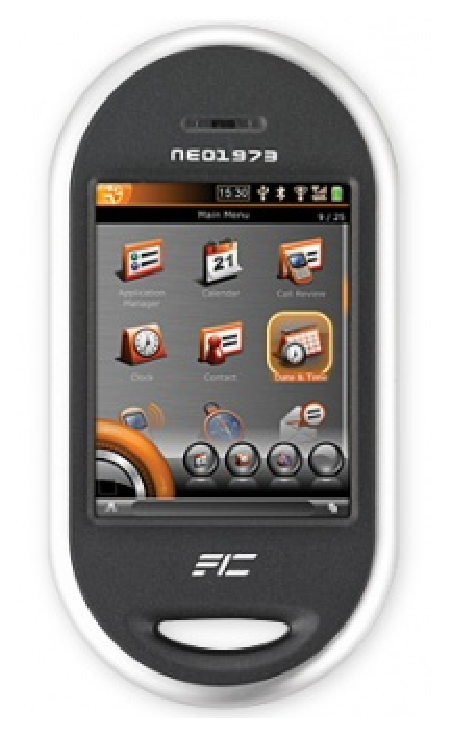
\includegraphics[bb=0 0 200 337,width=1.7in]{neo1973.eps}
% neo1973.eps: 300dpi, width=1.69cm, height=2.85cm, bb=0 0 200 337
	\caption{OpenMoko hardware}
	\label{fig:neo1973}
\end{figure}

%

Furthermore, it may be possible to get funding for a student to investigate this topic. Google sponsors a Summer of Code (SoC) initiative which funds students to spend a summer contributing to any one of a list of projects. The list of project is reviewed and prioritized by a number of open source organizations. In 2007, the project to integrate the GPSTk into the OpenMoko was listed, but not chosen by an SoC sponsored recipient \cite{summerofcodemainsite,summerofcodeopenmokogpstk}. If Google again sponsors a SoC for 2008, the GPSTk and OpenMoko projects would help support a student interested in this project.


\section*{Summary}

After three years since its public release, the GPSTk continues to amass new contributions and new developers. The third year required the GPSTk team to consider new ways to collaborate with developers distributed on a global scale. The project website became a primary means to provide dynamic documentation and to host user questions. The code repository was restructured to accommodate innovation while preserving core functionality. Applications were added to support processes that are key to GNSS research: range measurement validation, and simulation of GNSS signal tracking. Both student and professional projects continue to choose the GPSTk as a processing basis.

\section*{Acknowledgments}

The authors would like to acknowledge support from Applied Research Laboratories, The University of Texas at Austin, and the U.S. Federal Aviation Administration. The authors would also like to recognize the developers who have contributed both code and time to the project. In particular Chris Keuthe at the University of Calgary for his support of the make system, and Dr. Martin Vermeer at TKK, for his broad support of the project. GPSTk users have motivated development discussions and provide descriptions of their work. This includes Ulla Kallio at TKK and Massimo Burcheri at FGAN. Drs. Lightsey, Buckley and Stearman at UT Austin, and many of their students, have provided feedback and numerous project reports as well.

%\begin{flushleft}

\bibliography{gpstk}
%\bibliographystyle{plain} % alphabetized
\bibliographystyle{unsrt}  % ordered by reference

%\end{flushleft}

\end{document}
